

\section{Results}
In this section, we will show the results of our experiments obtained. We will the comparison of the results between the supervised and the self-supervised version of the InfNet.

\subsection{Result for self-supervised InfNet}
 The result for our comparison between the baseline InfNet model and our self-supervised model can be seen in \ref{tab:single}, and \ref{tab:multi-weakprior}. The table is plotted with several metrics: F1, IoU, Recall, and Precision. 
 
 For the table that contains mean and error, the mean are calculated as:
 \begin{equation}
mean =  \frac{\sum_{i=1}^{N}Metric(\hat{y_i}, y_i)}{N}
 \end{equation}
 Where Metric refers to either \textit{F1, IoU, Recall, Precision.} N refers to the number of test data samples.
 The error is:
 \begin{equation}
error =  SE x 1.96
 \end{equation}
 where SE is the standard error of the test data samples for the metric multiplied by 1.96.
Note that Mean $\pm$Error is the 95\% confidence interval.
 
 We show several tables for our comparisons. \ref{tab:single} shows the result for the single segmentation InfNet. The single segmentation InfNet does not segment between ground-glass opacities or consolidation. The single segmentation will segment and represent all infected region as one. We can see that self-supervision can improve on the generalization and consistency in predicting the different CT lung images as they perform the best in terms of the error range. Even though the baseline single SInfNet performance has better mean values for F1, IoU, and Recall, the self-supervised approach helps to create robustness and consistency in the model itself to better handle outliers. We can see the results of the single segmentation in \ref{fig:single-comparison}. We can see that the baseline single SInfNet overestimated the infected region of an outlier in the segmentation result in the figure in the last row. The self-supervised SInfNet did a better job at predicting outliers where its prediction is more closely related to the ground truth than the baseline single SInfNet.
 
 \begin{figure*}
 	\centering
 	\small
 	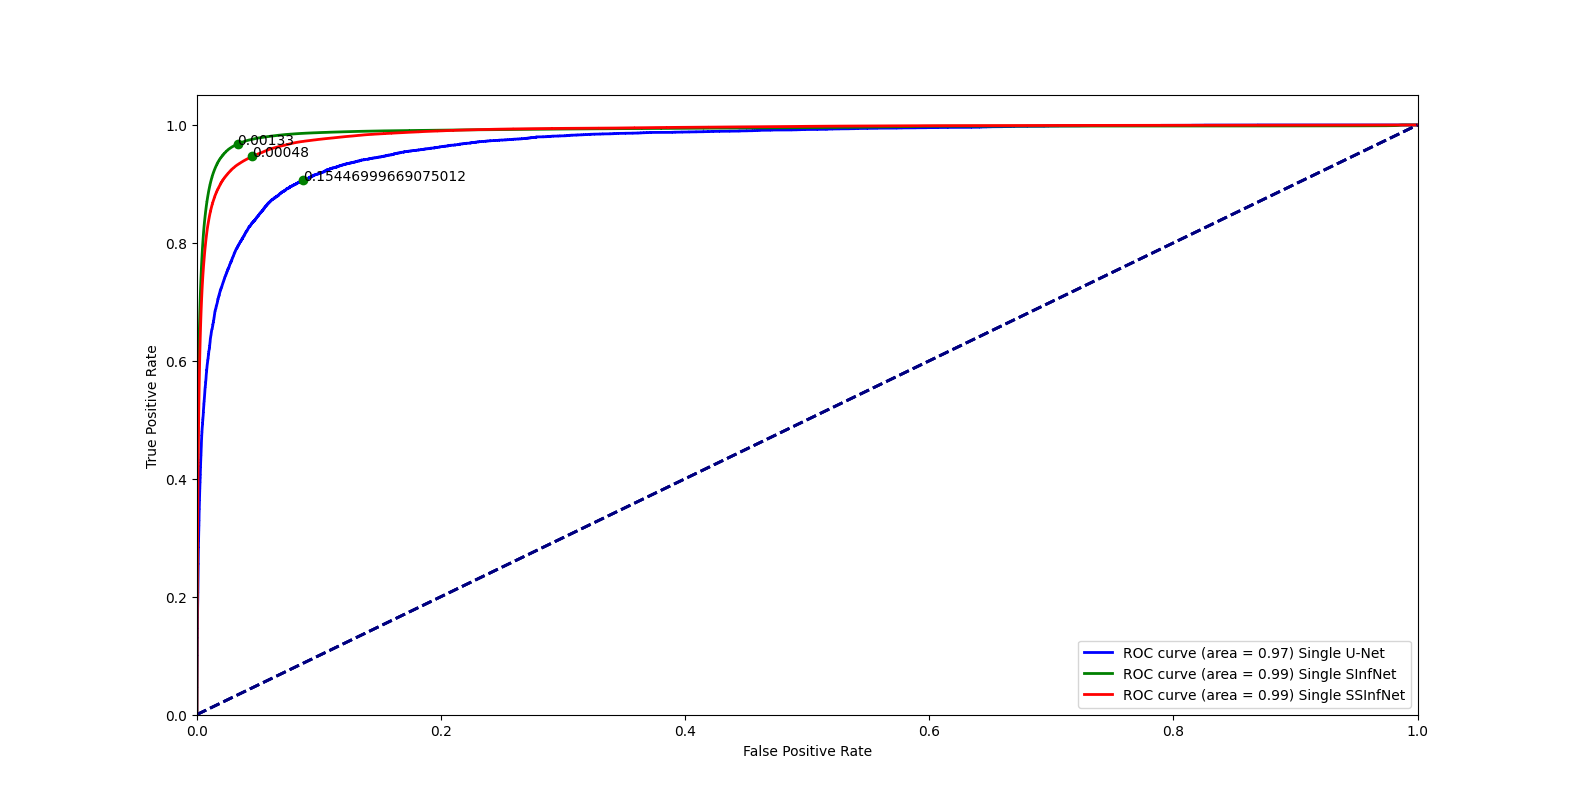
\includegraphics[width=\linewidth]{single_rocs.png}
 	\caption{ROC comparison of different networks.}
 	\label{fig:single_rocs}
 \end{figure*}
 
 \begin{table*}[!ht]
 	\centering
 	\begin{tabular}{| c | c || c c c c c ||}
 		\hline
 		Methods & & F1 & IoU & Recall & Precision & AUC \\ \hline
 		Single SInfNet &  Mean & \textbf{0.39} & \textbf{0.29} & \textbf{0.83} & 0.33 & \textbf{0.9909} \\ \cline{2-7}
 		& Error & $\pm$ 0.059 & $\pm$ 0.053 & $\pm$ \textbf{0.069} & $\pm$0.057  & $\pm$0.032 \\ \hline
 		Single Self-SInfNet &  Mean & 0.38 & 0.27 & 0.75 & 0.33 & 0.9883  \\ \cline{2-7}
 		& Error & $\pm$0.056 & $\pm$0.049 &$\pm$0.077  & $\pm$0.053 & $\pm$  0.010 \\ \hline
 		Single Self-SInfNet + data aug &  Mean & 0.30 & 0.20 & 0.72 & 0.28 &  0.9795 \\ \cline{2-7}
 		& Error & $\pm$ \textbf{0.050}  & $\pm$  \textbf{0.039} & $\pm$ 0.085 & $\pm$\textbf{0.045} & $\pm$ \textbf{0.006}  \\ \hline
 	\end{tabular}
 	\caption{Quantitative result for comparison between Single segmentation InfNet and self-supervised single segmentation InfNet in the test set.}
 	\label{tab:single}
 \end{table*}
 
 \begin{figure*}
 	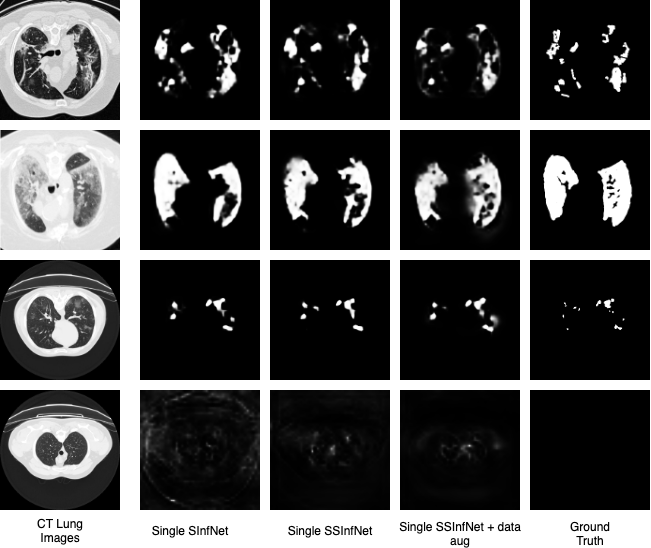
\includegraphics[width=\linewidth]{comparison_single.png}
 	\caption{Comparison of single segmentation between different networks.}
 	\label{fig:single-comparison}
 \end{figure*}

 \ref{tab:multi-weakprior} shows the result for the comparison between multiple segmentation InfNet. As the multiple segmentation InfNet requires a CT lung image concatenate with a prior as input where the prior is the segmentation of the infected region of the CT lung without considering the location of ground-glass opacities or consolidation. The prior represents the infected region as a whole. The prior is obtained by running prediction of the infected region by the single segmentation InfNet on the CT lung images of the test set. Then the prior is fed together with the CT lung image from the test set into the multiple segmentation InfNet to obtain the result. As the baseline InfNet achieves the best performing single InfNet, we use the prediction of the prior obtained from the baseline InfNet to be fed into the multi segmentation InfNet with the CT lung images. The self-supervised Multi InfNet was able to achieve a higher performance than the baseline Single InfNet. However, to further improve our self-supervised Multi InfNet, we added focal loss and lookahead optimizer. The improvement of the self-supervised Multi InfNet improved and has the highest performance comparing to the other networks. We can see the segmentation result in \ref{fig:multi-weakprior-comparison}.  
 
 \begin{table*}[!h]
 	\centering
 	\small
 	\begin{tabular}{| c | c || c c c c || c c c c |}
 		\hline
 		& &\multicolumn{4}{c||}{Ground-Glass Opacity} & \multicolumn{4}{c|}{Consolidation}\\ \cline{3-10}
 		Methods & & F1 & IoU & Recall & Precision & F1 & IoU & Recall & Precision \\\hline
 		U-Net & Mean & \textbf{0.45} & \textbf{0.33} & 0.43 & \textbf{0.59} & 0.13 & 0.08 & 0.12 & 0.18 \\ \cline{2-10}
 		& Error & $\pm$ 0.066 & $\pm$0.055& $\pm$0.07& $\pm$0.076& \textbf{$\pm$0.055}& \textbf{$\pm$0.037}& \textbf{$\pm$0.058}& $\pm$0.076 \\ \hline
 		SInfNet & Mean & 0.38 & 0.27 & 0.58 & 0.41 & 0.29 & 0.22 & 0.61 & 0.31  \\ \cline{2-10}
 		& Error & \textbf{$\pm$0.054} & \textbf{$\pm$0.042} & \textbf{$\pm$0.065} & $\pm$0.058 & $\pm$0.078 & $\pm$0.068 & $\pm$0.099 & $\pm$0.084  \\ \hline \hline
 		
 		\vtop{\hbox{\strut SSInfNet}\hbox{\strut }} & Mean & 0.36 & 0.26 & 0.56 & 0.4 & 0.31 & 0.25 & 0.56 & 0.38 \\ \cline{2-10}
 		& Error & $\pm$0.055 & $\pm$0.043 & $\pm$0.067 & $\pm$0.059 & $\pm$0.087 & $\pm$0.076 & $\pm$0.114 & $\pm$0.097 \\ \hline \hline
 		
 		\vtop{\hbox{\strut SSInfNet+}\hbox{\strut focal loss+}\hbox{\strut lookahead}} & Mean & 0.43 & 0.31 & 0.58 & 0.48 & \textbf{0.46} & \textbf{0.36} & 0.56 & \textbf{0.56} \\ \cline{2-10}
 		& Error & $\pm$0.057 & $\pm$0.046 & $\pm$0.072 & $\pm$0.059 & $\pm$0.096 & $\pm$0.088 & $\pm$0.11 & $\pm$0.101 \\ \hline \hline \hline
 		
 		
 		& &\multicolumn{4}{c||}{Background} & \multicolumn{4}{c|}{Overall}\\ \cline{3-10}
 		Methods & & F1 & IoU & Recall & Precision & F1 & IoU & Recall & Precision \\\hline
 		U-Net & Mean & 0.89 & 0.80 & 0.996 & 0.804 & 0.49 & 0.41 & 0.52 & 0.52  \\ \cline{2-10}
 		& Error &  $\pm$0.012&  $\pm$0.02&  $\pm$0.002&  $\pm$0.02&  $\pm$0.044&  $\pm$0.037&  \textbf{$\pm$0.043}&  $\pm$0.057 \\ \hline
 		SInfNet & Mean & 1.0 & 0.99 & 0.99 & 1.0 & 0.55 & 0.5 & \textbf{0.73} & 0.57   \\ \cline{2-10}
 		& Error & $\pm$0.002 & $\pm$0.003 & $\pm$0.002 & $\pm$0.002 & \textbf{$\pm$0.044} & $\pm$0.038 & $\pm$0.055 & $\pm$0.048 \\ \hline
 		\vtop{\hbox{\strut SSInfNet}\hbox{\strut }} & Mean & 1.0 & 0.99 & 1.0 & 1.0 & 0.56 & 0.5 & 0.71 & 0.59 \\ \cline{2-10}
 		& Error & $\pm$0.002 & $\pm$0.003 & $\pm$0.002 & $\pm$0.002 & $\pm$0.048 & $\pm$0.041 & $\pm$0.061 & $\pm$0.053\\ \hline \hline

 		\vtop{\hbox{\strut SSInfNet+}\hbox{\strut focal loss+}\hbox{\strut lookahead}} & Mean &1.0 & 0.99 & 0.99 & 1.0 & \textbf{0.63} & \textbf{0.55} & 0.71 & \textbf{0.68} \\ \cline{2-10}
 		& Error & $\pm$0.002 & $\pm$0.003 & $\pm$0.002 & $\pm$0.002 & $\pm$0.052 & $\pm$0.046 & $\pm$0.061 & $\pm$0.054\\ \hline \hline \hline
 		
 	\end{tabular}
 	\caption{Quantitative result of Ground-glass Opacities \& Consolidation on the test data set. Prior is obtained from the single segmentation InfNet}
 	\label{tab:multi-weakprior}
 \end{table*}

  \begin{figure*}
 	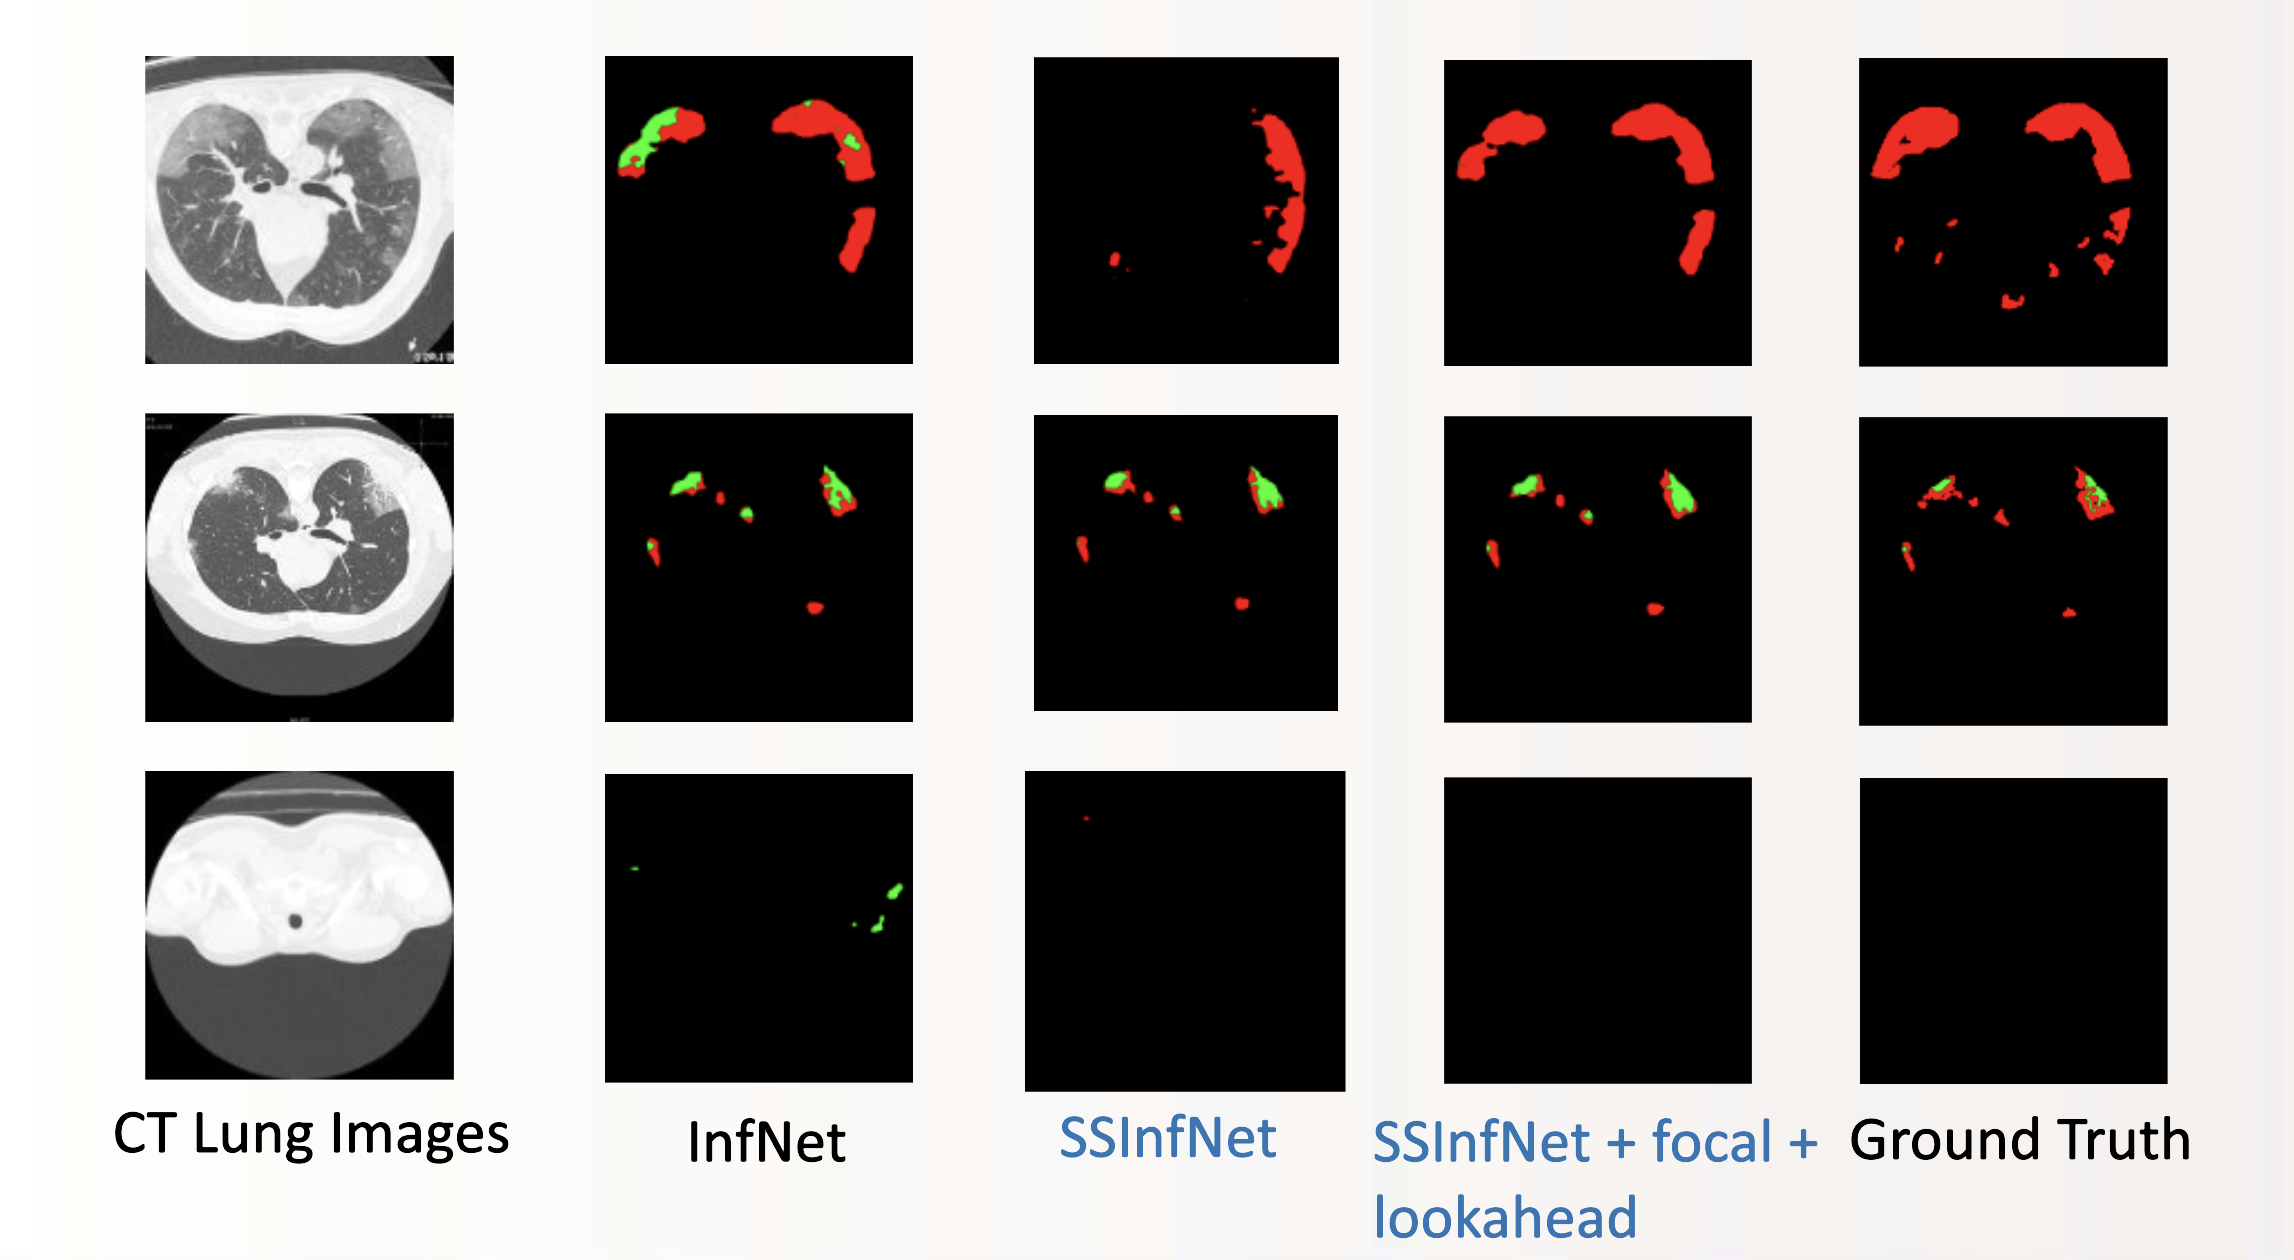
\includegraphics[width=\linewidth]{comparison_multi_weakprior.png}
 	\caption{Comparison of multi segmentation between different networks with prior generated from single InfNet.}
 	\label{fig:multi-weakprior-comparison}
 \end{figure*}
